% !TEX TS-program = lualatex
% !BIB TS-program = biber
\DocumentMetadata{
    lang=en,
    pdfstandard=ua-2,
    tagging=on,
    tagging-setup={
        math/setup={mathml-AF,mathml-SE},
        extra-modules={verbatim-mo},
    }
}
%% Options
% * bibstyle: biblatex bibliography style (keyword argument)
% * nocopyright: Disable copyright notice
% * nohyperref: Disable hyperlinks
% * ragged: Use ragged right edge rather than justified text (better for accessibility)
% * thesis: Master's thesis rather than dissertation
\documentclass{authesis}

%%%%%%%%%%%%%%%%%%%%%%%%%%%%%%%%%%%%%%%%%%%%%%%%%%
%%%%%%%%%%%%%%%%%%%% PACKAGES %%%%%%%%%%%%%%%%%%%%
%%%%%%%%%%%%%%%%%%%%%%%%%%%%%%%%%%%%%%%%%%%%%%%%%%
% fontsetup can slow down compilation, so it is disabled by default
% uncomment these commands to use a system font like Arial rather than default TeX sans-serif
%\usepackage{fontsetup}
%\setsansfont{Arial}

% If using math unicode-math is required.
\usepackage{unicode-math}

% If using figures, alt text is required. For example:
%  \includegraphics[alt={Alt text...}]{image.png}
\usepackage{graphicx}

% Bibliography (uses biblatex with biber as backend)
% Set the bibliography style using the bibstyle option of the class.
% Most other options can be changed here using
% \ExecuteBibliographyOptions{}
\addbibresource{./references.bib}

% Footnotes
\usepackage[bottom]{footmisc}
%%%%%%%%%%%%%%%%%%%%%%%%%%%%%%%%%%%%%%%%%%%%%%%%%%

%%%%%%%%%%%%%%%%%%%%%%%%%%%%%%%%%%%%%%%%%%%%%%%%%%
%%%%%%%%%%%%%%%%%%% TITLE PAGE %%%%%%%%%%%%%%%%%%%
%%%%%%%%%%%%%%%%%%%%%%%%%%%%%%%%%%%%%%%%%%%%%%%%%%
\title{Coffee Consumption Among Graduate Students Writing Dissertations}

\author{Alice Ascher}

% specify degree if other than Doctor of Philosophy or Master of Science
%\degreetype{Doctor of Education}

% date of graduation
\date{May 14, 2025}

% up to 6 keywords
\keywords{coffee, caffeine, academic writing}

% one entry per committee member
\committee{
\committeemember{Bob Barnard, Chair, Professor of Nutritional Sciences}
\committeemember{Charlie Clarke, Associate Professor of Nutritional Sciences with a Really Really Really Really Really Really Long Title}
\committeemember{Dan Drower, Professor of Nutritional Sciences}
\committeemember{Eve Earlsfield, Professor of English}
}
%%%%%%%%%%%%%%%%%%%%%%%%%%%%%%%%%%%%%%%%%%%%%%%%%%

\begin{document}

\begin{frontmatter}
\maketitle

\begin{abstract}
The abstract is a concise summary of the contents of the thesis or dissertation.
A reasonable length for the abstract is 350 words for a dissertation and 150 words
for a thesis. The abstract is an important guide to potential readers searching for
information about your topic.
\end{abstract}

\begin{aidisclosure}
% If AI tools were used, complete and use the following statement only:
%In the preparation of this {\thesistype}, the following Artificial Intelligence (AI) tools
%were used: [list specific tools]. These tools were used primarily to [describe specific
%functions]. The author acknowledges full responsibility for the intellectual content of this
%work and has ensured that all AI-assisted sections have been reviewed and revised for
%accuracy and appropriate academic style. All AI-generated content was reviewed and
%validated for relevance, appropriateness, and accuracy before incorporation into the
%final document to maintain scholarly integrity of this research.
%
% If no AI tools were used, use the following statement only:
In the preparation of this {\thesistype}, no Artificial Intelligence (AI) tools were used.
\end{aidisclosure}

\begin{accessibilitydisclosure}
In the preparation of this {\thesistype}, the following digital
accessibility tools were used to ensure this document complies with federal
requirements: [list specific software/tools]. The author acknowledges full responsibility
for the intellectual content of this work and has made a good faith effort to comply with
digital accessibility requirements in publishing, wherein the nature of the content does
not significantly change in order to do so. Furthermore, all content has been reviewed
and revised to meet these requirements prior to final publication.
\end{accessibilitydisclosure}

\begin{acknowledgements}
I am grateful to my parents for their support.
\end{acknowledgements}

\tableofcontents

\listoftables

\listoffigures

% List of abbreviations, entered like a table
\begin{listofabbreviations}
AU & Auburn University \\
UA & University of Alabama
\end{listofabbreviations}

\end{frontmatter}

% Chapters
\chapter{Coffee Consumption Mathematics}

Coffee extraction occurs when hot water is poured over coffee grounds, causing
desirable compounds such as caffeine, carbohydrates, lipids, melanoidins and
acids to be extracted from the grounds.

Extraction yield refers to the solubles dissolved during brewing. This is often
expressed as a percentage of the coffee's mass. It is also known as solubles
yield or simply extraction. The extraction yield percentage describes the mass
transferred from coffee grounds to water, expressed as a percentage of the
initial mass of the grounds. It is given by eq.~\eqref{ch1:eq:extraction_yield}.

\begin{equation}
    Y = \frac{M_2 \cdot t}{M_1}
    \label{ch1:eq:extraction_yield}
\end{equation}

where $Y$ is the extraction yield expressed as a percentage, $t$ is the total
dissolved solids expressed as a percentage of the final beverage, $M_1$ is the
mass of the grounds in grams, and $M_2$ is the final beverage's mass in grams.
This means that an extraction yield of 20\% can be obtained by brewing 18 grams
of coffee, resulting a 36-gram final beverage with a $t$ of 10\%. Yield can also
be expressed as total dissolved solids, or parts-per-million (ppm).

Here is a subscript $x_1$ and superscript $x^2$. Here is a subsubscript $x_{y_1}$,
a supersuperscript $x^{y^1}$, and the others $x_{y^2}$ and $x^{y_2}$.
% set graphics path for each chapter with figures if organizing figures per chapter
\graphicspath{ {./chapter/02} }
\chapter{Coffee Berries}

A coffee bean is a seed from the Coffea plant and the source for coffee (Figure \ref{ch2:fig:coffee_berries}). This
fruit is often referred to as a coffee cherry, but unlike the cherry, which
usually contains a single pit, it is a berry most commonly found having two
seeds with their flat sides together.

\begin{figure}
    \centering
    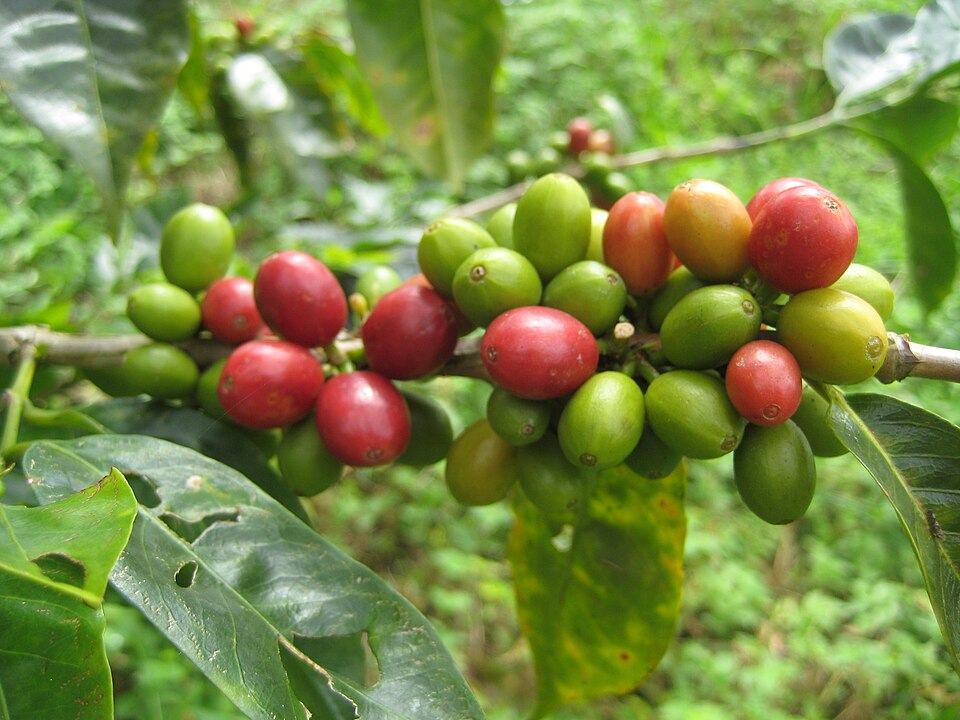
\includegraphics[width=0.6\textwidth,alt={Multiple red and green coffee
    berries clustered together on coffee tree branches}]{
        Clumps_of_coffee_berries_growing_on_a_tree_by_Brian_Smith.jpg
    }
    \caption{Clumps of coffee berries growing on a tree (Photo by Brian Smith)}
    \label{ch2:fig:coffee_berries}
\end{figure}

\section{Characteristics of Coffee Berries}

The two most economically important varieties of coffee plants are the arabica
and the robusta; approximately 60\% of the coffee produced worldwide is arabica
and some 40\% is robusta (Table \ref{ch2:tab:coffee_species}).

\begin{table}
    \centering
    \caption{Common Coffee Species Comparison}
    \medskip
    \label{ch2:tab:coffee_species}
    \renewcommand{\arraystretch}{1.5}
    \tagpdfsetup{table/header-columns={1},table/header-rows={1}}
    \begin{tabular}{|>{\bfseries}l|l|l|}
        \hline
        Species & \textbf{Flavor Profile} & \textbf{Global Production} \\
        \hline
        Arabica & Smooth, complex, with fruit notes & 60\% \\
        \hline
        Robusta & Strong, bitter, earthy & 40\% \\
        \hline
    \end{tabular}
\end{table}
\pagebreak

\subsection{Key information}

Table \ref{ch2:tab:coffee_characteristics} summarizes key information about coffee berries:

\begin{table}
    \centering
    \caption{Key Characteristics of Coffee Berries}
    \medskip
    \label{ch2:tab:coffee_characteristics}
    \renewcommand{\arraystretch}{1.5}
    \tagpdfsetup{table/header-columns={1}}
    \begin{tabular}{|>{\bfseries}p{2in}|p{4in}|}
        \hline
        Color at Ripeness & Bright red, yellow or pink depending on variety \\
        \hline
        Size & Approximately 15 mm in diameter \\
        \hline
        Weight & 300--330 mg dry \\
        \hline
        Seeds per Berry & Typically 2 seeds; 10--15\% are peaberries (single seed) \\
        \hline
        Time to Maturity & 6--11 months depending on variety and growing conditions \\
        \hline
        Caffeine Content & 1.0--2.5\% by dry weight \\
        \hline
        Growing Conditions & Altitudes of 600--2,200 meters; temperatures of 15--24°C \\
        \hline
        Shelf Life (Fruit) & 2--3 weeks if left on tree after ripening \\
        \hline
    \end{tabular}
\end{table}
\chapter{Coffee Chemistry}

Caffeine is a central nervous system (CNS) stimulant of the
methylxanthine class and is the most commonly consumed psychoactive substance
globally.

Some people\footnote{Over 90\% of American adults consume caffeine daily, see ref.~\citenum{SleepFoundation1}.}
drink beverages containing caffeine to relieve or prevent drowsiness and to
improve cognitive performance. To make these drinks, caffeine is extracted by
steeping the plant product in water, a process called infusion.

Overall population mean coffee consumption was stable from 2003 to 2012
\cite{LOFTFIELD20161762}.
\chapter{Coffee Charts: A Chapter with a Really Really Really Really Really Really Really Really Really Really Really Really Long Title}

\section{A Section with a Really Really Really Really Really Really Really Really Really Really Really Long Title}
Data visualization is an important aspect of understanding coffee consumption
patterns and production statistics. The following chart displays typical daily
coffee consumption at different times (see Appendix \ref{appA:coffee_survey}).

\subsection{A Subsection with a Really Really Really Really Really Really Really Really Really Really Really Long Title}
The following line chart illustrates the trend of coffee consumption throughout
a week. There is a noticeable increase in consumption during the middle of the
week, peaking on Thursday and Friday, followed by a decline over the weekend.


% Bibliography
\printbibliography[heading=bibintoc,title={References}]

% Appendices
\appendix
\chapter{Coffee Survey}

\section{Survey Questions}
\label{appA:coffee_survey}

\begin{enumerate}
    \item How many cups of coffee do you consume on an average weekday?
    \item How many cups of coffee do you consume on an average weekend day?
    \item How many cups of coffee do you consume during deposit week?
    \item How many cups of coffee do you consume after deposit week?
\end{enumerate}
\chapter{Coffee Survey Data}

\section{Survey Respondent Statistics}
A total of 100 graduate students participated in the coffee consumption survey.
The average age of respondents was 28 years, with a range of 22 to 35 years.

\section{Survey Opinions}
When asked about their coffee preferences, 70\% of respondents indicated a
preference for dark roast coffee, while 30\% preferred light roast.

\end{document}
